\section{E. Коровы в стойла}
\textit{Условие задачи:} \par
На прямой расположены стойла, в которые необходимо расставить коров так, чтобы минимальное расcтояние между коровами было как можно больше.\\
\textit{Пояснение к примененному алгоритму:} \par
Необходимо перебрать возможные расстояния между стойлами, попробовать расставить коров, и выбрать максимальное.
Так как ограничение по времени 0.1 секунд, то алгоритм перебора O($N^2$) не подойдёт ($N_{max}$ = $10^5$):
Поэтому я применил бинпоиск по дистанции - нахожу возможную дистанцию, проверяю циклом, могу ли разместить коров с этой дистанцией.
Если да - пробую взять больше, если нет - меньше, и так, пока две границы бинпоиска не будут содержать в себе максимальную дистанцию,
с которой можно разместить (левая), и минимальную, с которой нельзя (правая).
Сложность алгоритма получается O(Nln($N^2$)).
\begin{figure}[H]
    \centering
    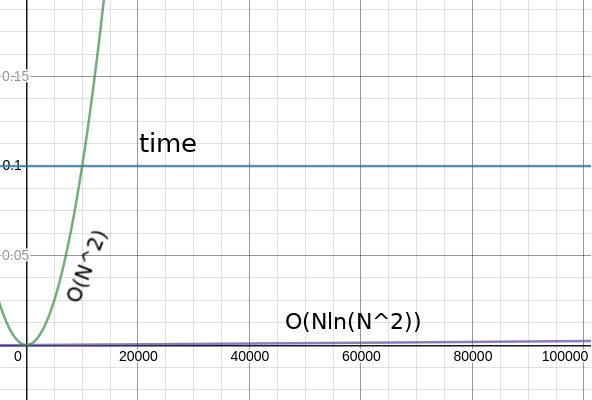
\includegraphics[scale=0.4]{img/saveaspng}
\end{figure}
\BgThispage
\newpage
\textit{Код:}
\small
\begin{center}
    \begin{verbatim}
bool try_placement(vector<int64_t> coords, int64_t distance,
               uint16_t cows_count);

int main() {
  uint32_t N, K;
  cin >> N >> K;
  vector<int64_t> coordinates(N);
  int64_t Z;
  for (size_t i = 0; i < N; i++) {
    cin >> Z;
    coordinates[i] = Z;
  }
  int64_t L = 0;
  int64_t R = coordinates.back();
  while (R - L > 1) {
    int64_t dist = (R + L) / 2;
    bool res = try_placement(coordinates, dist, K);
    if (res) {
      L += (R - L) / 2;
    } else {
      R -= (R - L) / 2;
    }
  }
  cout << L << endl;
  return 0;
}

bool try_placement(vector<int64_t> coords, int64_t distance,
                   uint16_t cows_count) {
  size_t iter = 0;
  int64_t place = coords[iter];
  for (size_t i = 1; i < cows_count; i++) {
    while (coords[iter] < place + distance) {
      iter++;
      if (iter == coords.size())
        return false;
    }
    place = coords[iter];
  }
  return true;
}

    \end{verbatim}
\end{center}
\normalsize
\BgThispage
\newpage


\section{F. Число}
\textit{Условие задачи:} \par
Вася написал на длинной полоске бумаги большое число и решил похвастаться своему старшему брату Пете этим достижением.
Но только он вышел из комнаты, чтобы позвать брата, как его сестра Катя вбежала в комнату и разрезала полоску бумаги на
несколько частей. В результате на каждой части оказалось одна или несколько идущих подряд цифр.
Теперь Вася не может вспомнить, какое именно число он написал. Только помнит, что оно было очень большое. Чтобы утешить
младшего брата, Петя решил выяснить, какое максимальное число могло быть написано на полоске бумаги перед разрезанием. Помогите ему! \par
\textit{Пояснение к примененному алгоритму:} \par
Читаю все числа и сортирую их: рассматривая каждую пару чисел в строковом формате, формирую два варианта их расположения - $s_1$$s_2$ и $s_2$$s_1$,
после чего посимвольно сравниваю их, как только встречается в одной из строк цифра больше, чем в другой на той же позиции - определяется расположение чисел.
Сложность: O($ln(N^2)$)\par
\textbf{Ex}: 201 и 215. Сравниваем 201215 и 215201. На второй итерации 1>0, поэтому 215 будет стоять впереди.\par
\textit{Код:}
\small
\begin{center}
  \begin{verbatim}
    bool comp(const string &el1, const string &el2) {
    string variant1 = el1 + el2;
    string variant2 = el2 + el1;
    for (size_t i = 0; i < variant1.size(); i++) {
        char symbol_from_var1 = variant1.at(i);
        char symbol_from_var2 = variant2.at(i);
        if (symbol_from_var1 > symbol_from_var2) return true;
        else if (symbol_from_var1 < symbol_from_var2) return false;
    }
    return false;
}

int main() {
    vector<string> input;
    string line;
    while (cin >> line) {
        input.push_back(line);
    }
    sort(input.begin(), input.end(), comp);
    for (const string &s: input) {
        cout << s;
    }
    return 0;
}

  \end{verbatim}
\end{center}
\normalsize
\BgThispage
\newpage


\section{G. Кошмар в замке}
\textit{Условие задачи:} \par
Ходят легенды, что пока Аврора спала, ей снилось, что она ходит по разным местам: леса, поля, города и сёла.
И вот однажды она наткнулась на пещеру, в которой сидел мудрец. Когда мудрец поднял на Аврору глаза, он изрёк: «Дорогая Аврора!
Ты уже годами скитаешься по этим землям. Я хочу предложить тебе задачку. Вот тебе строка s. Каждая буква из алфавита имеет
свой вес $c_i$. Вес строки, которую ты можешь получить из s многократным обменом любых двух букв, вычисляется так: для каждой
буквы алфавита посчитай максимальное расстояние между позициями, в которых стоит эта буква и перемножь его с весом этой буквы.
Принеси мне строку максимально возможного веса, и я тебе расскажу, в чём смысл жизни».\par
\textit{Пояснение к примененному алгоритму:} \par
Так как для искомого максимума считается одно максимальное расстояние между парами для одного вида букв, очевидно, что
выгоднее всего располагать по краям буквы с наибольшим "весом", и, чем меньше "вес" буквы, тем ближе к центру.
Читаем строку и значения для каждой буквы. Значения записываем сразу парой<буква, значение>, а после сортируем массив пар
по значению в порядке неубывания. Далее перебираем список пар от большего к меньшему: если находим букву из текущей пары в строке, начинаем поиск с конца такой же буквы.
Если пара найдена - перемещаем их на границы строки, и сдвигаем указатель границы на один (чтобы следующую пару, значение которой будет меньше текущей, поставить перед текущей).\par
Сложность алгоритма: сортировка - O($Nln(N)$) + перебор O($N^2$) $\approx$ O($N^2$).
\BgThispage
\newpage
\textit{Код:}
\small
\begin{center}
    \begin{verbatim}
        bool comp(pair<char, ::uint32_t> p1, pair<char, ::uint32_t> p2) {
    return p1.second > p2.second;
}

int main() {
    string line;
    cin >> line;
    vector<pair<char, uint32_t>> values(26);
    const char literals_begin = 'a';
    for (int i = 0; i < 26; i++) {
        uint32_t value;
        cin >> value;
        values[i] = make_pair(literals_begin + i, value);
    }
    sort(values.begin(), values.end(), comp);
    size_t replace_counts = 0;
    for (pair<char, ::uint32_t> p: values) {
        size_t pos1 = 0;
        size_t pos2 = 0;
        for (size_t i = replace_counts; i < line.size() - replace_counts; i++) {
            if (line[i] == p.first) {
                pos1 = i;
                for (size_t j = line.size() - replace_counts - 1; j > i; j--) {
                    if (line[j] == p.first) {
                        pos2 = j;
                        break;
                    }
                }
                break;
            }
        }
        if (pos2 != 0) {
            string s1 = line.substr(pos1, 1);
            string s2 = line.substr(pos2,1);
            line.erase(pos1, 1);
            line.erase(pos2 - 1, 1);
            line.insert(replace_counts, s1);
            line.insert(line.size() - replace_counts, s2);
            replace_counts++;
        }
    }
    cout << line << endl;
    return 0;
}
    \end{verbatim}
\end{center}
\normalsize
\BgThispage
\newpage

\section{H. Магазин}
\textit{Условие задачи:} \par
У Билла большая семья: трое сыновей, девять внуков. И всех надо кормить. Поэтому Билл раз в неделю ходит в магазин.
Однажды Билл пришел в магазин и увидел, что в магазине проводится акция под названием «каждый k-й товар бесплатно».
Изучив правила акции, Билл выяснил следующее. Пробив на кассе товары, покупатель получает чек. Пусть в чеке n товаров,
тогда n/k округленное вниз самых дешевых из них достаются бесплатно.Например, если в чеке пять товаров за 200, 100, 1000,
400 и 100 рублей, соответственно, и k = 2, то бесплатно достаются оба товара по 100 рублей, всего покупатель должен заплатить 1600 рублей.
Билл уже выбрал товары, и направился к кассе, когда сообразил, что товары, которые он хочет купить, можно разбить на несколько
чеков, и благодаря этому потратить меньше денег. Помогите Биллу выяснить, какую минимальную сумму он сможет заплатить за
выбранные товары, возможно разбив их на несколько чеков.\par
\textit{Пояснение к примененному алгоритму:} \par
Для наглядности рассмотрю пример:\\
1000 700 500 300 200 100 (k=3). В таком чеке выгода будет 300 рублей. Максимизируя выгоду, вынесу в отдельный чек два самых
дорогих товара, так как их стоимость не срезать никак, и выберу самый дорогой товар из оставшихся, чтобы срезать максимально
возможную общую стоимость. Получится (1000, 700, 500) и (300, 200, 100), выгода 600. Таким образом, для получения максимальной выгоды
необходимо отсортировать список цен товаров по возрастанию, и разбивать их на тройки по чекам, пока это возможно.
Реализованный алгоритм: читаем список чисел, сортируем в порядке неубывания, и пробегаемся по списку товаров от начала,
считая каждый k-й в выгоду.\par
Сложность алгоритма: сорт - O($Nln(N)$) + подсчёт выгоды - O(N) $\approx$ O($Nln(N)$)
\BgThispage
\newpage
\textit{Код:}
\small
\begin{center}
    \begin{verbatim}
        bool comp(uint16_t a, uint16_t b) {
    return a>b;
}

int main() {
    size_t n;
    size_t k;
    cin >> n >> k;
    vector<uint16_t> prices(n);
    for (size_t i=0; i<n; i++) {
        uint16_t price;
        cin >> price;
        prices[i] = price;
    }
    sort(prices.begin(), prices.end(), comp);
    uint64_t cost=0;
    for (size_t i=0; i<prices.size(); i++) {
        if ( (i+1) % k != 0) {
            cost+=prices[i];
        }
    }
    std::cout << cost << std::endl;
    return 0;
}
    \end{verbatim}
\end{center}
\BgThispage
